% =====================================================================
% Figure 1 (corrected) — Overall dataflow of INS-HDGS-CMT
% Standalone: compile directly, or \input{} into the manuscript.
% Fix vs. previous version: ROI is shown as a feature DERIVED from
% eye-tracking gaze (dwell histogram), not a separate input modality.
% Matches models/ins_hdgs_cmt.py forward pass.
% =====================================================================
\documentclass[tikz,border=8pt]{standalone}
\usepackage{tikz}
\usetikzlibrary{arrows.meta,positioning,fit,backgrounds,calc}

\begin{document}
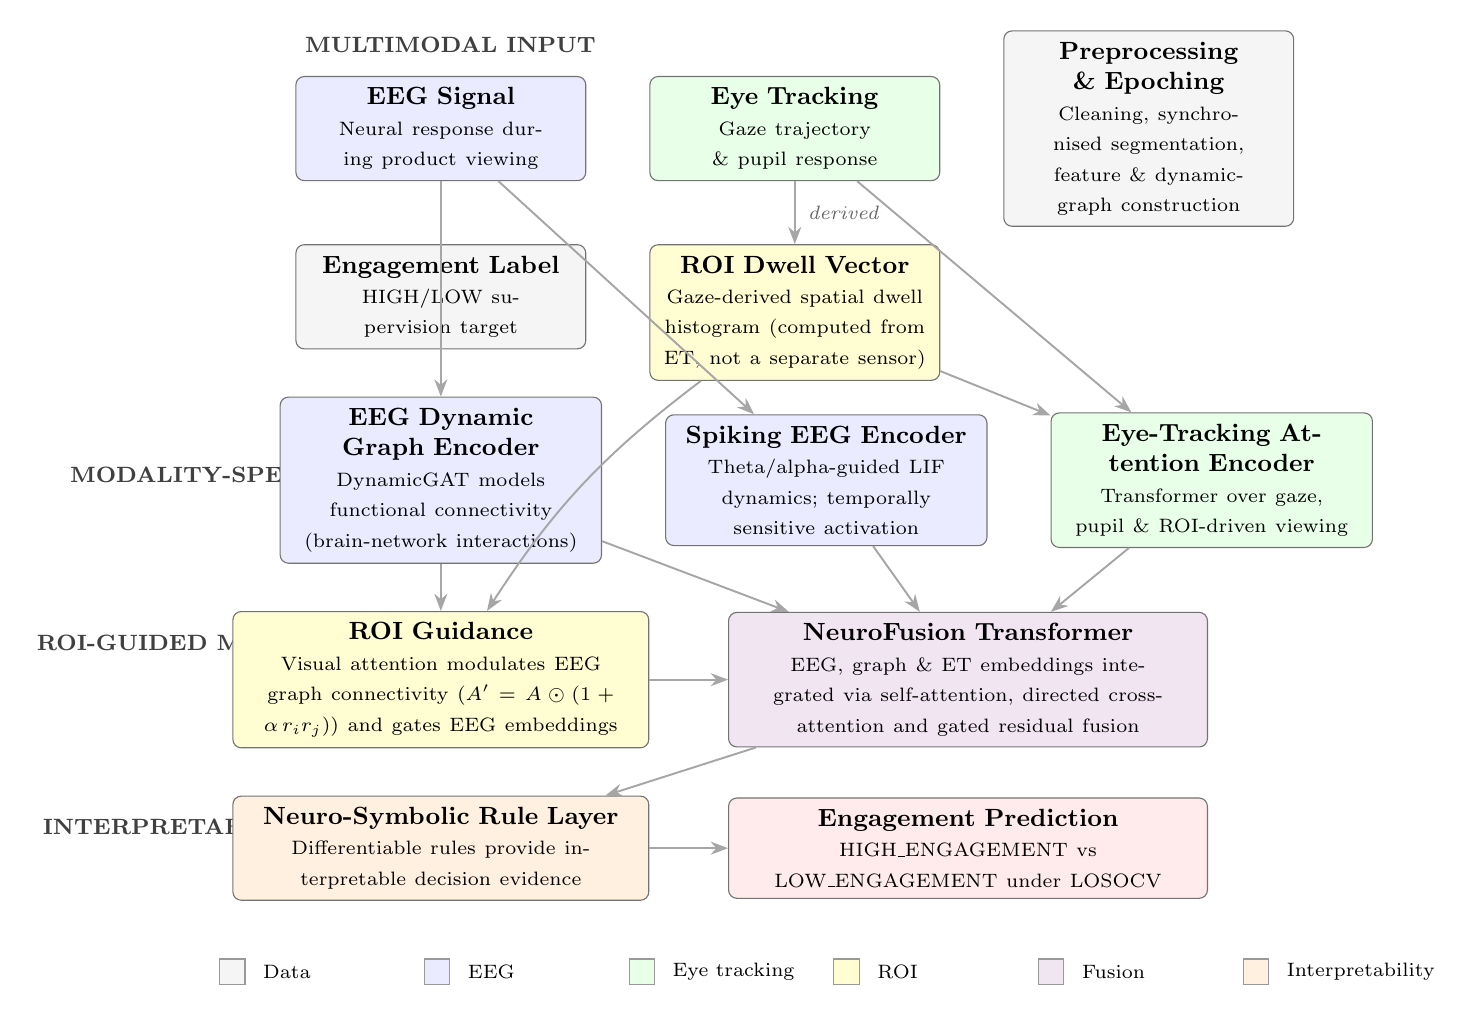
\begin{tikzpicture}[
  font=\small,
  >={Stealth[length=2.2mm]},
  box/.style={rounded corners=3pt, draw=black!55, line width=0.4pt,
              align=center, inner sep=4pt, text width=34mm, minimum height=12mm},
  data/.style ={box, fill=gray!8},
  eeg/.style  ={box, fill=blue!8},
  et/.style   ={box, fill=green!9},
  roi/.style  ={box, fill=yellow!18},
  fus/.style  ={box, fill=violet!10},
  intp/.style ={box, fill=orange!12},
  pred/.style ={box, fill=red!8},
  flow/.style ={->, line width=0.7pt, gray!70},
  tier/.style ={font=\bfseries\footnotesize, text=black!75},
  node distance=6mm and 8mm,
]

% ---------- Tier labels (left) ----------
\node[tier] (t1) {MULTIMODAL INPUT};

% ---------- Inputs ----------
\node[eeg,  below=4mm of t1.west, anchor=north west] (eeg) {\textbf{EEG Signal}\\\scriptsize Neural response during product viewing};
\node[et,   right=of eeg]  (et)  {\textbf{Eye Tracking}\\\scriptsize Gaze trajectory \& pupil response};
\node[data, right=of et]   (prep){\textbf{Preprocessing \& Epoching}\\\scriptsize Cleaning, synchronised segmentation, feature \& dynamic-graph construction};

% ROI now DERIVED from eye tracking
\node[roi, below=8mm of et] (roi){\textbf{ROI Dwell Vector}\\\scriptsize Gaze-derived spatial dwell histogram (computed from ET, not a separate sensor)};
\draw[flow] (et) -- (roi) node[midway,right=1pt,font=\scriptsize\itshape,text=black!60]{derived};

\node[data, below=8mm of eeg] (label){\textbf{Engagement Label}\\\scriptsize HIGH/LOW supervision target};

% ---------- Tier 2: encoders ----------
\node[tier, below=12mm of roi.south, anchor=north] (t2lab) {};
\node[tier] at ($(eeg.west|-roi.south)+(0,-12mm)$) (t2) {MODALITY-SPECIFIC ENCODING};

\node[eeg, below=6mm of label, text width=38mm] (gat)
  {\textbf{EEG Dynamic Graph Encoder}\\\scriptsize DynamicGAT models functional connectivity (brain-network interactions)};
\node[eeg, right=of gat, text width=38mm] (snn)
  {\textbf{Spiking EEG Encoder}\\\scriptsize Theta/alpha-guided LIF dynamics; temporally sensitive activation};
\node[et,  right=of snn, text width=38mm] (eten)
  {\textbf{Eye-Tracking Attention Encoder}\\\scriptsize Transformer over gaze, pupil \& ROI-driven viewing};

\draw[flow] (eeg)  -- (gat);
\draw[flow] (eeg)  -- (snn);
\draw[flow] (et)   -- (eten);
\draw[flow] (roi)  -- (eten);

% ---------- Tier 3: ROI-guided fusion ----------
\node[tier] at ($(gat.west|-gat.south)+(0,-10mm)$) (t3) {ROI-GUIDED MULTIMODAL FUSION};

\node[roi, below=6mm of gat, text width=50mm] (roig)
  {\textbf{ROI Guidance}\\\scriptsize Visual attention modulates EEG graph connectivity ($A'=A\odot(1+\alpha\,r_i r_j)$) and gates EEG embeddings};
\node[fus, right=10mm of roig, text width=58mm] (fuse)
  {\textbf{NeuroFusion Transformer}\\\scriptsize EEG, graph \& ET embeddings integrated via self-attention, directed cross-attention and gated residual fusion};

\draw[flow] (roi)  to[bend right=10] (roig);
\draw[flow] (gat)  -- (roig);
\draw[flow] (gat)  -- (fuse);
\draw[flow] (snn)  -- (fuse);
\draw[flow] (eten) -- (fuse);
\draw[flow] (roig) -- (fuse);

% ---------- Tier 4: decision ----------
\node[tier] at ($(roig.west|-roig.south)+(0,-10mm)$) (t4) {INTERPRETABLE DECISION};

\node[intp, below=6mm of roig, text width=50mm] (ns)
  {\textbf{Neuro-Symbolic Rule Layer}\\\scriptsize Differentiable rules provide interpretable decision evidence};
\node[pred, right=10mm of ns, text width=58mm] (pred)
  {\textbf{Engagement Prediction}\\\scriptsize HIGH\_ENGAGEMENT vs LOW\_ENGAGEMENT under LOSOCV};

\draw[flow] (fuse) -- (ns);
\draw[flow] (ns)   -- (pred);

% ---------- Legend ----------
\begin{scope}[shift={($(ns.south west)+(0,-9mm)$)}]
  \foreach \i/\c/\txt in {0/gray!8/Data, 1/blue!8/EEG, 2/green!9/Eye tracking,
                          3/yellow!18/ROI, 4/violet!10/Fusion, 5/orange!12/Interpretability}{
    \node[draw=black!40, fill=\c, minimum width=3.2mm, minimum height=3.2mm,
          inner sep=0pt] (l\i) at (\i*26mm,0) {};
    \node[right=1mm of l\i, font=\scriptsize] {\txt};
  }
\end{scope}

\end{tikzpicture}
\end{document}
